\documentclass[a4paper,12pt]{article}

% polyglossia should go first!
\usepackage{polyglossia} % multi-language support
\setmainlanguage{russian}
\setotherlanguage{english}
\PolyglossiaSetup{english}{indentfirst=true}
\PolyglossiaSetup{russian}{indentfirst=true}

\defaultfontfeatures{Mapping=tex-text} % for converting "--" and "---"
\setmainfont{CMU Serif}
\setsansfont{CMU Sans Serif}
\setmonofont{CMU Typewriter Text}

\usepackage{minted}
\newcommand{\inputmintedbr}[2]{\inputminted[breaklines=true]{#1}{#2}}

% Опционно, требует  apt-get install scalable-cyrfonts.*
% и удаления одной строчки в cyrtimes.sty
% Сточку не удалять!
% \usepackage{cyrtimes}

% Картнки и tikz
\usepackage{graphicx}
\usepackage{tikz}
\usetikzlibrary{snakes,arrows,shapes}


% Некоторая русификация.
%\usepackage{misccorr}
\usepackage{indentfirst}
\renewcommand{\labelitemi}{\normalfont\bfseries{--}}

% Увы, поля придётся уменьшить из-за листингов.
\topmargin -1cm
\oddsidemargin -0.5cm
\evensidemargin -0.5cm
\textwidth 17cm
\textheight 24cm

\sloppy

% Оглавление в PDF
\usepackage[
bookmarks=true,
colorlinks=true, linkcolor=black, anchorcolor=black, citecolor=black, menucolor=black,filecolor=black, urlcolor=black,
unicode=true
]{hyperref}

% Для исходного кода в тексте
\newcommand{\Code}[1]{\textbf{#1}}

%\usepackage{verbatim}
%\usepackage{fancyvrb}
%\fvset{frame=leftline, fontsize=\small, framerule=0.4mm, rulecolor=\color{darkgray}, commandchars=\\\{\}}
%\renewcommand{\theFancyVerbLine}{\small\arabic{FancyVerbLine}}

%tables
\usepackage{tabu}
\usepackage{multirow}

\title{Отчёт по лабораторной работе \\ <<Система доменных имён>>}
\author{Гребенюк Александр Андреевич}

\begin{document}

\maketitle

\clearpage
\tableofcontents

\clearpage
\section{Настройка системы DNS}

\subsection{Топология сети}

Топология сети и использыемые IP-адреса показаны на рис.~\ref{fig:network}.

\begin{figure}
\centering
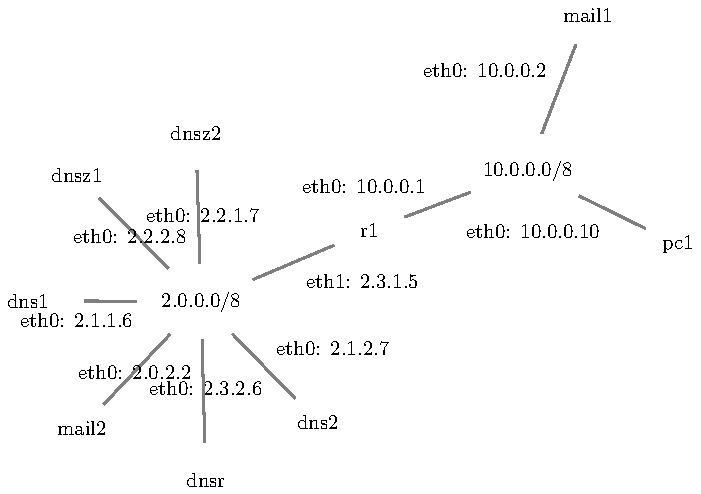
\includegraphics[width=\textwidth]{includes/network_gv.pdf}
\caption{Топология сети}
\label{fig:network}
\end{figure}

\subsection{Структура службы доменных имён}

Структура авторитетных серверов доменных имён показана на рис.~\ref{fig:dns}.

\begin{figure}
\centering
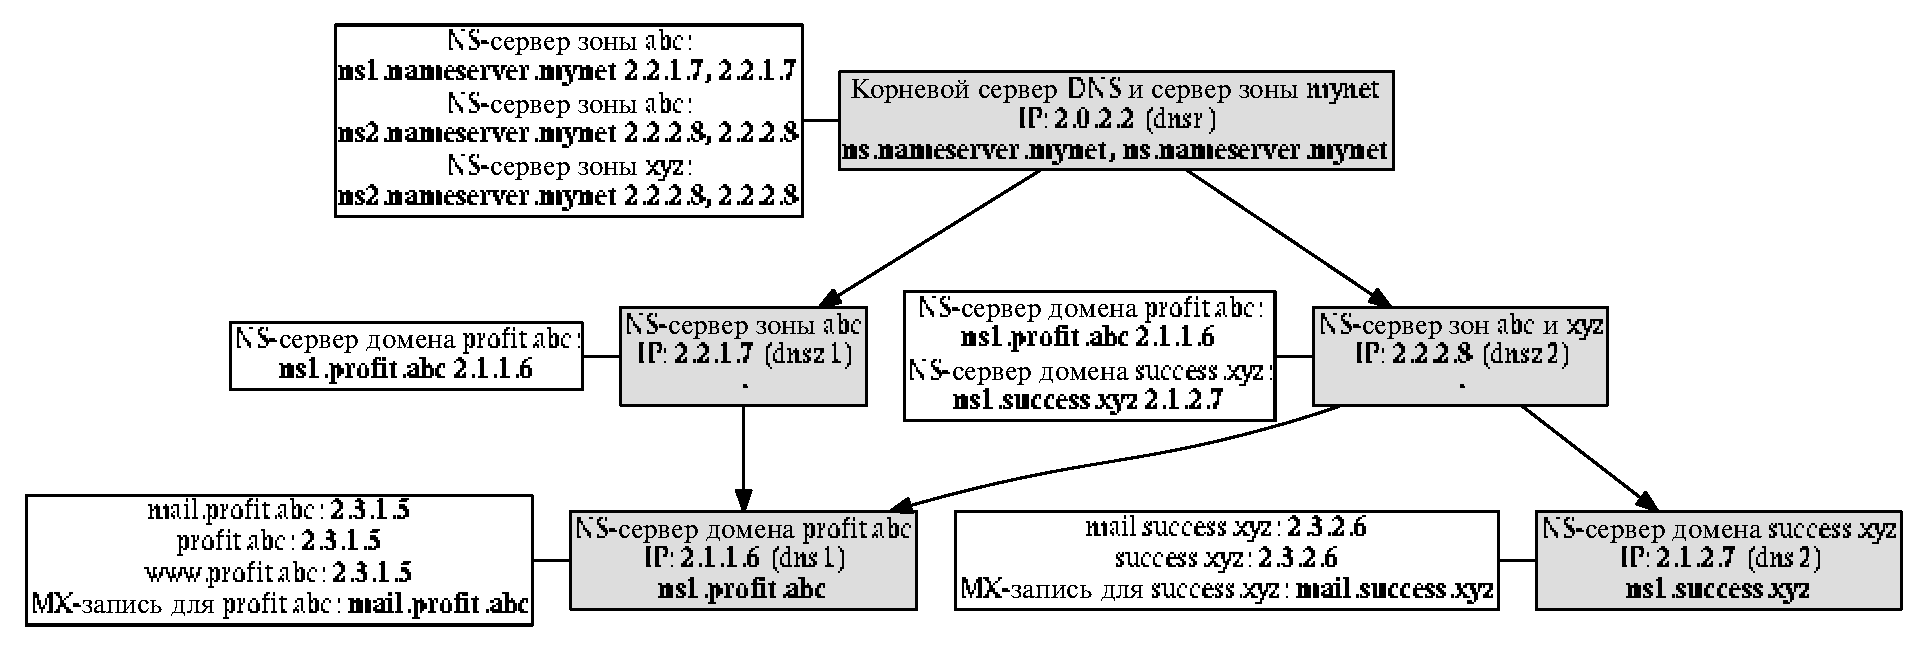
\includegraphics[width=\textwidth]{includes/dns_gv.pdf}
\caption{Структура службы доменных имён}
\label{fig:dns}
\end{figure}

\subsection{Прочие настройки}

Кеширующие DNS-серверы
\begin{itemize}
\item \textbf{r1}
\end{itemize}

Развёрнутые SMTP-серверы и используемые ими кеширующие DNS-серверы.
\begin{itemize}
\item \textbf{mail1} использует сервер на \textbf{r1};
\item \textbf{mail2} использует сервер на \textbf{r1};
\end{itemize}


\clearpage
\section{Проверка настройки службы доменных имён}

\subsection{Проверка настройки записи типа A для домена mail.profit.abc}

\textbf{dnsr}
\inputmintedbr{text}{../../results/dnsr.dig}


\clearpage
\textbf{dnsz1}
\inputmintedbr{text}{../../results/dnsz1.dig}


\clearpage
\textbf{dnsz2}
\inputmintedbr{text}{../../results/dnsz2.dig}


\clearpage
\textbf{dns1}
\inputmintedbr{text}{../../results/dns1.dig}


\clearpage
Итоговая проверка: опрашиваем кеширующий DNS-сервер.
\inputmintedbr{text}{../../results/r1.dig}


Пинг с \textbf{r1}
\inputmintedbr{text}{../../results/ping.log}


\clearpage
\section{Проверка работы почтовой системы}

\subsection{Проверка MX-записи для домена \textbf{profit.abc}}

С узла \textbf{mail2} отправили письмо на локальный SMTP-сервер для адресата с адресом \textbf{root@profit.abc}

\inputmintedbr{text}{../../results/mail2.send.log}

На машине с доменным именем \textbf{mail1} появилось доставленное письмо.
\inputmintedbr{text}{../../results/mail1.recv.log}

Таким образом, доменная запись типа MX для домена \textbf{profit.abc} настроена верно.

\clearpage
\subsection{Проверка MX-записи для домена \textbf{success.xyz}}

С узла \textbf{mail1} отправили письмо на локальный SMTP-сервер для адресата с адресом \textbf{root@success.xyz}

\inputmintedbr{text}{../../results/mail1.send.log}

На машине с доменным именем \textbf{mail2} появилось доставленное письмо.
\inputmintedbr{text}{../../results/mail2.recv.log}

Таким образом, доменная запись типа MX для домена \textbf{success.xyz} настроена верно.

\end{document}
